\begin{figure}
	\floatbox{figure}[\FBwidth]
	{
		\caption{The representation of women in top economics journals}\label{figure5}
	}
	{
	\begin{minipage}{0.3\textwidth}
		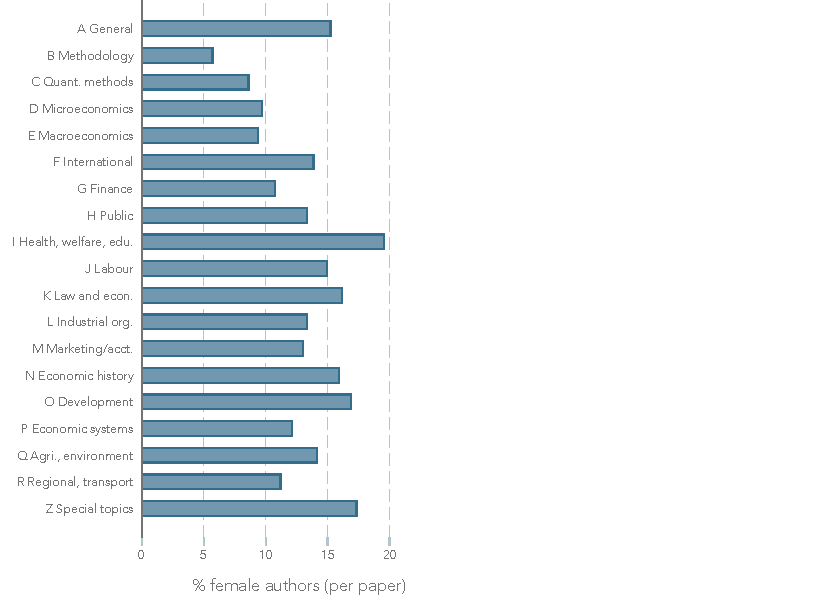
\includegraphics[trim=0.25cm 0cm 6.7cm 0cm, clip, width=1.1\linewidth]{0-images/generated/Figure-2-jel.pdf}
	\end{minipage}
	\begin{minipage}{0.65\textwidth}
		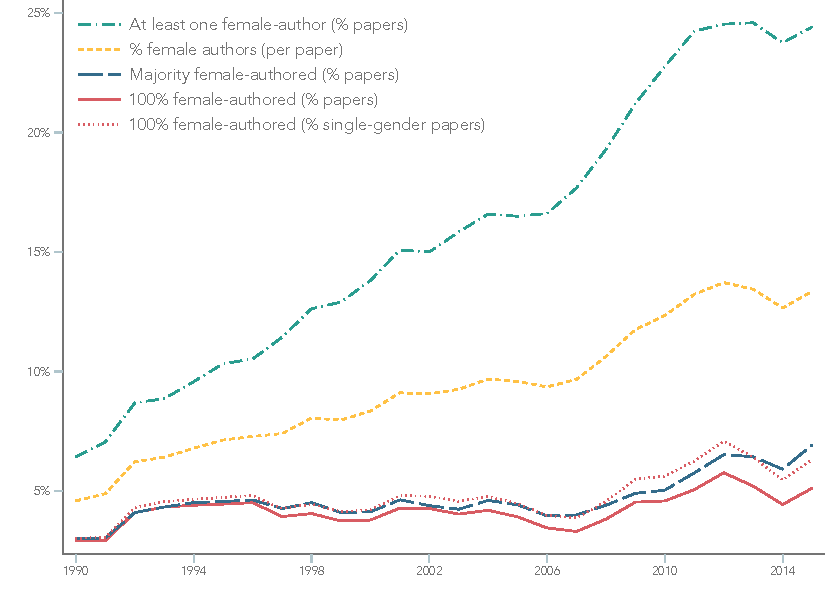
\includegraphics[width=0.95\linewidth]{0-images/generated/Figure-2-time.pdf}
	\end{minipage}
		\floatfoot{\tiny \textit{Notes}. Sample 5,211 articles. Graphs illustrate the representation of female authors in articles published in top-four economics journals. Figure on the left is the average share of female authors per paper broken down by primary \textit{JEL} category; figure on the right displays the evolution of papers' gender composition over time as five-year moving averages.}
	}
\end{figure}